\chapter{Организационно-экономический раздел}
Организация и планирование процесса разработки программного обеспечения предусматривает выполнение следующих задач:
\begin{enumerate}[1.]
\item формирование состава выполняемых работ и группировка их по стадиям разработки;
\item расчет трудоемкости выполнения работ;
\item расчет количества исполнителей;
\item построение сетевого графика;
\item разработка календарного графика работ;
\item Анализ структуры затрат проекта;
\item Оценка экономической целесообразности проекта;
\end{enumerate}

\section{Основные этапы разработки программного продукта}
Разработку программного продукта разбивают на следующие стадии в соответствии с ЕСПД ГОСТ 19102-77:
\begin{enumerate}[1.]
\item \textbf{Техническое задание.} Постановка задач. Определение пакета прикладных программ, состава и структуры информационной базы. Выбор языков программирования. Предварительный выбор методов выполнения работы. Разработка календарного плана выполнения работ.
\item \textbf{Эскизный проект.} Предварительная разработка структуры входных и выходных данных. Разработка общего описания алгоритмов решения задач. Разработка пояснительной записки. Согласование и утверждение эскизного проекта.
\item \textbf{Технический проект.} Разработка алгоритмов решения задач. Разработка пояснительной записки. Согласование и утверждение технического проекта. Разработка структуры программы. Разработка программной документации и передача ее для включения в технический проект. Внесение правок в структуры, анализ и определение формы представления входных и выходных данных. Выбор конфигурации технических средств.
\item \textbf{Рабочий проект.} Комплексная отладка задач и сдача в опытную эксплуатацию. Разработка проектной документации. Программирование и отладка программ. Описание контрольного примера. Разработка программной документации. 
\item \textbf{Внедрение.} Подготовка и передача программной документации для сопровождения с оформлением соответствующего акта. Передача программной продукции в фонд алгоритмов и программ. Проверка алгоритмов и программ решения задач, корректировка документации после опытной эксплуатации программного продукта.
\end{enumerate}

Анализируя требования ГОСТ, можно предложить следующее распределение работ по этапам:
\begin{enumerate}[1.]
\item Разработка технических требований, предъявляемых к разрабатываемому ПО и проведение исследований заданной области.
\item Разработка алгоритмов работы ПО, выбор среды программирования.
\item Разработка программных модулей (написание кода).
\item Тестирование и отладка разрабатываемого ПО.
\item Разработка документации.
\end{enumerate}

Этап внедрения отсутствует, так как разрабатываемое ПО будет внедряться силами заказчиков данного ПО без участия разработчиков.

\section{Расчет трудоемкости проекта}
Определим вероятные трудозатраты на выполнение данного проекта. Существует несколько методик определения трудозатрат, воспользуемся определением с помощью экспертных оценок. Для этой цели было опрошено четверо экспертов-разработчиков в области сетевых технологий.

В таблице~\ref{table:expert_marks} приведены оценки экспертов:

\begin{table}
\centering
\caption{Экспертные оценки}
\label{table:expert_marks}
\begin{tabular} {| c | c |} 
\hline
Эксперт 1 & 500\\
\hline
Эксперт 2 & 400\\
\hline
Эксперт 3 & 650\\
\hline
Эксперт 4 & 700\\
\hline
\end{tabular}
\end{table}

Общие затраты труда на разработку определим следующим образом:
\begin{equation}
Q_{P} = \sum_{i}t_i,
\end{equation}
где $t_{i}$ - затраты труда на выполнение i-го проекта.

Используя метод экспертных оценок, вычислим ожидаемую продолжительность работ T каждого этапа по формуле:
\begin{equation}
T = \frac{3 \cdot T_{MIN} + 2 \cdot T_{MAX}} {5} = \frac{3 \cdot 400 + 2 \cdot 700} {5} = 520,
\end{equation}
где $T_{MIN}$ - минимальная продолжительность работ, $T_{MAX}$ - максимальная продолжительность работ;

Продолжительности работ назначаются в соответствии с экспертными оценками, а ожидаемая продолжительность работы рассчитывается как математическое ожидание для $\beta$-распределения.

Полный перечень работ с разделением по этапам приведен в таблице~\ref{table:all_works}.
\begin{table}
\caption{Перечень работ}
\label{table:all_works}
\begin{tabular} {| p{0.15\textwidth} | p{0.08\textwidth} | p{0.3\textwidth} | p{0.1\textwidth} | p{0.1\textwidth} | p{0.1\textwidth} | p{0.09\textwidth} |} 
\hline
Этап & № & Содержание & $T_{MIN}$, & $T_{MAX}$, & T, & T, \\
& работы & работы & чел/часы & чел/часы & чел/часы & чел/дни\\
\hline
\multirow{4}{\hsize}{Разработка технических требований}
& 1 & Согласование списка поддерживаемых протоколов & 8 & 8 & 8 & 1\\
\cline{2-7}
& 2 & Разработка и утверждение ТЗ & 16 & 36 & 24 & 3\\
\cline{2-7}
& 3 & Анализ предметной области и существующих решений & 20 & 30 & 24 & 3\\
\cline{2-7}
& 4 & Анализ фреймворка DPDK и его возможностей & 16 & 16 & 16 & 2\\
\hline
\multirow{3}{\hsize}{Описание структур данных и алгоритмов}
& 5 & Разработка файла конфигурации: синтаксис, поддерживаемые действия, допустимые значения & 48 & 68 & 56 & 7\\
\cline{2-7}
& 6 & Разработка алгоритмов обнаружения протоколов & 72 & 92 & 80 & 10\\
\hline
\multirow{2}{\hsize}{Разработка программных модулей}
& 7 & Реализация модуля работы с файлом конфигурации & 60 & 70 & 64 & 8\\
\cline{2-7}
& 8 & Реализация главного модуля обработки сетевого трафика & 90 & 145 & 112 & 14\\
\hline
\multirow{3}{\hsize}{Тестирование и отладка ПО}
& 9 & Тестирование функциональности & 32 & 52 & 40 & 5\\
\cline{2-7}
& 10 & Тестирование производительности & 24 & 24 & 24 & 3 \\
\hline
Разработка документации & 12 & Написание программной и эксплуатационной документации & 66 & 81 & 72 & 9\\
\hline
\end{tabular}
\end{table}

Итого: $Q_{\textup{Р}} = Q_{\textup{ОЖ}} = 65 \textup{чел/дней} = 520 \textup{чел/час}$

\section{Определение численности исполнителей}
Средняя численность исполнителей определяется по формуле:
\begin{equation}
N = \frac{Q_{P}} {F},
\end{equation}
где F - фонд рабочего времени и определяется по формуле:
\begin{equation}
F = \sum_{i}^r F_{Mi} = \sum_{i}^r (D_{\textup{о}} - D{ \textup{в}} - D_{\textup{п}}),
\end{equation}
где $F_{Mi}$ - фонд времени в текущем i-том месяце и вычисляется для каждого месяца с учетом количества праздников $D_{\textup{о}}$, выходных $D_{\textup{в}}$ и праздничных $D_{\textup{п}}$ дней.

На реализацию проекта отведено r = 3 месяца рабочего времени при односменной работе с продолжительностью рабочего времени 8 часов. В таблице~\ref{table:time_fond} приведены сведения, необходимые для вычисления фонда времени для каждого месяца и итоговые результаты вычислений.
\begin{table}
\caption{Месячный фонд времени}
\label{table:time_fond}
\begin{tabular} {| p{0.1\textwidth} | p{0.2\textwidth} | p{0.15\textwidth} | p{0.15\textwidth} | p{0.15\textwidth} | p{0.15\textwidth} |} 
\hline
Месяц & Количество & Количество & Количество & Фонд & Фонд\\
& дней & выходных & праздничных & времени & времени \\
& & дней & дней & $F_{Mi}$,  дни & $F_{Mi}$, дни\\
\hline
Февраль & 29 & 8 & 1 & 20 & 159\\
\hline
Март & 31 & 9 & 1 & 21 & 168\\
\hline
Апрель & 30 & 9 & 0 & 21 & 168\\
\hline
Итого & & & & 62 & 495\\
\hline
\end{tabular}
\end{table}

Таким образом, фонд рабочего времени проекта составляет  F = 495 часов.

Отсюда средняя численность исполнителей равна:
\begin{equation}
N = \frac{Q_{P}} {F} = \frac{520} {495} = 1.05
\end{equation}

Таким образом, по суммарным трудозатратам для завершения проекта в заданные сроки необходимо два исполнителя: инженер и программист. Учитывая специфику дипломного проекта, данные специалисты должны обладать знаниями в следующих областях:
\begin{itemize}
\item протоколы вычислительных сетей;
\item сетевое программирование;
\item высокопроизводительные информационные системы и комплексы;
\item разработка алгоритмов и архитектуры ПО;
\item тестирование ПО;
\item разработка документации;
\end{itemize}

\section{Построение сетевого графика}
Для определения временных затрат и трудоемкости разработки ПО используем метод сетевого планирования. Этот метод позволяет установить единой схемой связь между всеми работами в виде наглядного и удобного для восприятия изображения (сетевого графика), представляющего собой информационно-динамическую модель, позволяющую определить продолжительность и трудоемкость как отдельных этапов, так и всего комплекса работ в целом.

Составление сетевой модели включает в себя оценку степени детализации комплекса работ и определения логической связи между отдельными работами. С этой целью составляется перечень всех основных работ и событий. В перечне указываются кодовые номера событий, наименования событий в последовательности от исходного к завершающему, кодовые номера работ, перечень всех работ, причем подряд указываются все работы, которые начинаются после наступления данного события.

Основные событий и работы представлены в таблице~\ref{table:events_and_works}.
\begin{longtable}{| p{0.03\textwidth} | p{0.33\textwidth} | p{0.1\textwidth} | p{0.3\textwidth} | p{0.07\textwidth} | p{0.07\textwidth} |} 
\caption{Основные работы и события проекта}
\label{table:events_and_works}
\\ \hline
$N_{i}$  & Наименование события & Код & Работа & t, & t,\\
& & работы & & чел/ч & чел/д \\
\hline \endfirsthead
\subcaption{Продолжение таблицы~\ref{table:events_and_works}}
\\ \hline \endhead
\hline \subcaption{Продолжение на след. стр.}
\endfoot
\hline \endlastfoot

0 & Разработка ПО начата & 0-1 & Согласование списка поддерживаемых протоколов & 8 & 1\\
\hline
1 & Протоколы согласованы & 1-2 & Разработка и утверждение ТЗ & 24 & 3\\
\hline
2 & ТЗ разработано и утверждено & 2-3 & Анализ предметной области и существующих решений & 24 & 3\\
\hline
3 & Анализ существующих решений проведен & 3-4 & Анализ фреймворка DPDK & 16 & 2\\
\hline
4 & DPDK проанализирован & 4-5 & Разработка файла конфигурации & 56 & 7\\
\cline{3-6}
& & 4-6 & Разработка алгоритмов обнаружения & 80 & 10\\
\hline
5 & Описание файла конфигурации выполнено & 5-6 & Фиктивная работа & 0 & 0\\
\hline
6 & Алгоритмы разработаны & 6-7 & Реализация модуля конфигурации & 64 & 8\\
\hline
7 & Модуль файла конфигурации реализован & 7-8 & Реализация главного модуля & 112 & 14\\
\hline
8 & Главный модуль реализован & 8-9 & Тестирование функциональности & 40 & 5\\
\cline{3-6}
& & 8-10 & Тестирование производительности & 24 & 3\\
\hline
9 & Функциональность протестирована & 9-11 & Разработка документации & 72 & 9\\
\hline
10 & Производительность протестирована & 10-12 & Фиктивная работа & 0 & 0\\
\hline
11 & Документация разработана & 11-12 & Фиктивная работа & 0 & 0\\
\hline
12 & Разработка ПО завершена & - & - & - & -\\

\end{longtable}

Сетевой график приведен на рисунке~\ref{fig:netgraph}.
\begin{figure}
\centering
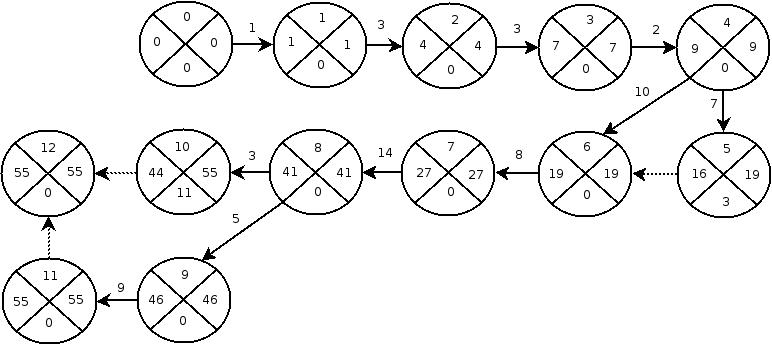
\includegraphics[scale=0.5]{pictures/netgraph}
\caption{Сетевой график}
\label{fig:netgraph}
\end{figure}

\section{Диаграмма Гантта}
Для иллюстрации последовательности проводимых работ на календарном графике приведена диаграмма Гантта (рисунок~\ref{fig:econom_gant}). По оси $X$ расположены календарные дни от начала проекта, а по оси $Y$ - выполняемые этапы работ.
\begin{figure}
\centering
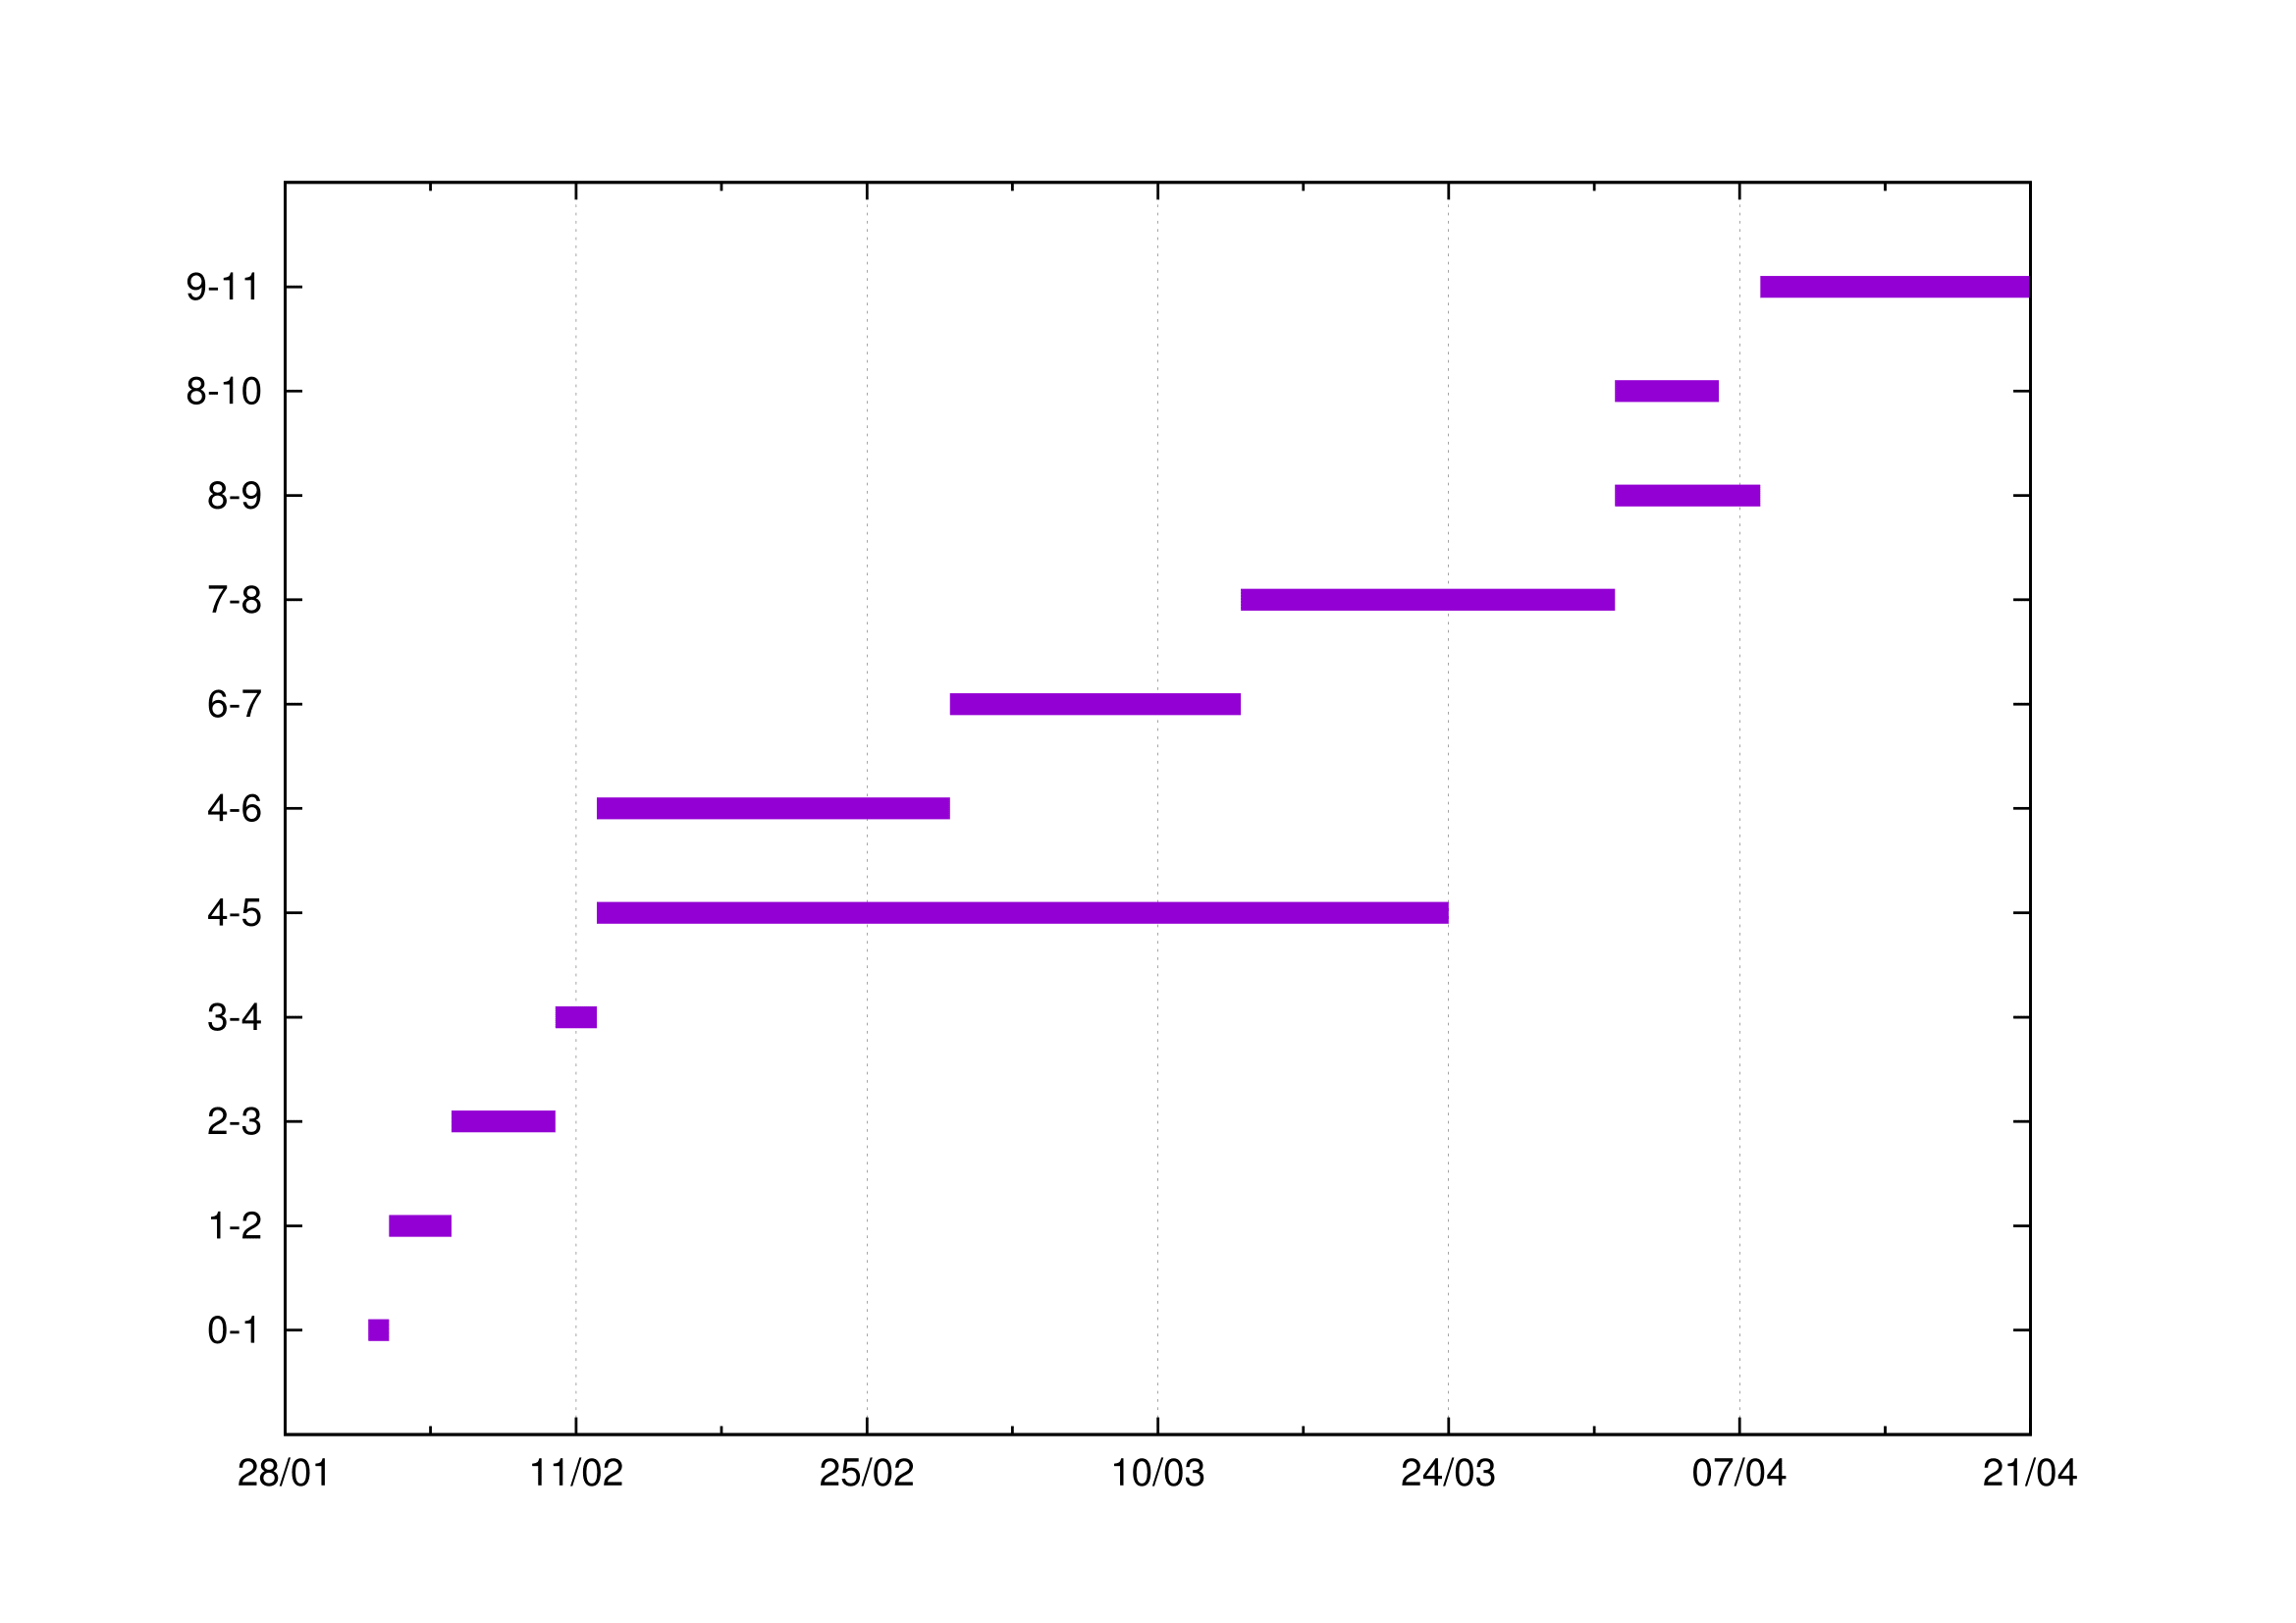
\includegraphics[scale=0.2]{pictures/gantt}
\caption{Диаграмма Гантта}
\label{fig:econom_gant}
\end{figure}

\begin{table}
\centering
\caption{Таблица занятости исполнителей}
\label{table:time_zan}
\begin{tabular} {| l | l | l | l |} 
\hline
Код работы &   Начало & Окончание & Исполнитель\\
\hline
0-1 & 02.02.16 & 02.02.16 & Программист\\
\hline
1-2 & 03.02.16 & 05.02.16 & Программист\\
\hline
2-3 & 08.02.16 & 10.02.16 & Программист\\
\hline
3-4 & 11.02.16 & 12.02.16 & Программист\\
\hline
4-5 & 15.02.16 & 24.03.16 & Программист\\
\hline
4-6 & 15.02.16 & 29.02.16 & Инженер\\
\hline
6-7 & 01.03.16 & 14.03.16 & Программист\\
\hline
7-8 & 15.03.16 & 01.04.16 & Программист\\
\hline
8-9 & 04.04.16 & 08.04.16 & Инженер\\
\hline
8-10 & 04.04.16 & 06.04.16 & Программист\\
\hline
9-11 & 11.04.16 & 21.04.16 & Инженер\\
\hline
\end{tabular}
\end{table}

\section{Анализ структуры и затрат проекта}
Затраты на выполнение проекта состоят из затрат на заработную плату исполнителям, затрат на закупку или аренду оборудования, затрат на организацию рабочих мест, и затрат на накладные расходы:
\begin{equation}
K = C_{\textup{ЗАРП}} + C_{\textup{ОБ}} + C_{\textup{ОРГ}} + C_{\textup{НАКЛ}},
\end{equation}
где $C_{\textup{ЗАРП}}$ - заработная плата исполнителей, $C_{\textup{ОБ}}$ - затраты на обеспечение необходимым оборудованием, $C_{\textup{ОРГ}}$ - затраты на организация рабочих мест, $C_{\textup{НАКЛ}}$ - накладные расходы.

\subsection{Затраты на выплату исполнителям заработной платы}
Затраты на выплату исполнителям заработной платы $C_{\textup{ЗАРП}}$ определяется следующим соотношением:
\begin{equation}
C_{\textup{ЗАРП}} = C_{\textup{З.ОСН}} + C_{\textup{З.ДОП}} + C_{\textup{З.ОТЧ}},
\end{equation}
где $C_{\textup{З.ОСН}}$ - основная заработная плата, $C_{\textup{З.ДОП}}$ - дополнительная заработная плата, $C_{\textup{З.ОТЧ}}$ - отчисления с заработной платы.

Расчет основной заработной платы при дневной оплате труда исполнителей проводится на основе данных по окладам и графику занятости исполнителей:
\begin{equation}
C_{\textup{З.ОСН}} = T_{\textup{ЗН}} \cdot O_{\textup{ДН}},
\end{equation}
где $O_{\textup{ДН}}$ - дневной оклад исполнителя, $T_{\textup{ЗН}}$ - число дней, отработанных исполнителем.

При 8-часовом рабочем дне $O_{\textup{ДН}}$ рассчитывается по формуле:
\begin{equation}
O_{\textup{ДН}} = \frac{O_{\textup{МЕС}} \cdot 8} {F_{M}},
\end{equation}
где $O_{\textup{МЕС}}$ - месячный оклад, $F_{M}$ - месячный фонд рабочего времени (приведен в таблице~\ref{table:time_fond}).

С учетом налога на доходы физических лиц размер месячного оклада увеличивается:
\begin{equation}
O_{\textup{МЕС}} = O \cdot (1 + \frac{H_{\textup{ДФЛ}}} {100}),
\end{equation}
где O - оклад, который позволит исполнителю заниматься проектом и который получен из информации кадровых агентств, $H_{\textup{ДФЛ}}$ - налог на доходы с физических лиц (13\%).

Предполагаемый размер заработной платы исполнителей был взят с интернет-портала www.hh.ru (03.05.2016). Расчет представлен в таблице~\ref{table:salary_of_executors} (размер оклада приведен с учетом налога на доходы с физических лиц).
\begin{table}
\caption{Оклады исполнителей}
\label{table:salary_of_executors}
\begin{tabular} {| l | l | l | l | l | l |} 
\hline
№ & Должность & "Чистый" & Дневной & Трудозатраты & Затраты на\\
&  & оклад, руб. & оклад, руб. & чел-день & зарплату, руб.\\
\hline
1 & Инженер & 100000 & 5478.79 & 24 & 131490.96\\
\hline
2 & Программист & 90000 & 4930.91 & 41 & 202167.31\\
\hline
3 & Итого & & & & 333658.27\\
\hline
\end{tabular}
\end{table}

Дополнительная заработная плата. Учитываются все выплаты непосредственным исполнителям за время, не проработанное на производстве, в том числе: оплата очередных отпусков, компенсации на недоиспользованный отпуск и др. Эти выплаты составляют 20\% от основной заработной платы:

$C_{\textup{З.ДОП}}$ = 0.2 $\cdot$ 333658.27 = 66731.6 руб.

Отчисления в пенсионный фонд, фонд социального страхования, занятости, на страховую медицины. Согласно нормативным документам, суммарные отчисления этой категории составляют 30\% от размеров заработной платы:

$C_{\textup{З.ОТЧ}}$ = (333658.27 + 66731.6) $\cdot$ 0.3 = 120116.96 руб.

\subsection{Затраты на оборудование}
Для организации рабочего процесса необходимо приобрести следующее:
%\item Ноутбук Asus K501Ux (58000 руб.)
%\item Ноутбук G50-80 (39000 руб.)
\begin{table}
\caption{Расходные материалы и оборудование}
\begin{tabular} {| l | l | l | l | l | l |} 
\hline
№ & Наименование & Ед. изм. & Кол-во & Цена за ед., руб. & Сумма\\
\hline
1 & Ноутбук Lenovo IdeaPad 100 15 & шт & 1 & 30000 & 30000\\
\hline
2 & Ноутбук Lenovo G50-80 & шт & 1 & 39000 & 39000\\
\hline
3 & Ручка шариковая синяя & шт & 4 & 68.50 & 274\\
& Pilot BPS-GP-EF & & & &\\
\hline
4 & Бумага Снегурочка & шт & 2 & 234 & 936\\
& (A4, 80 г/кв.м, белизна 146\% & & & &\\
& CIE, 500 листов) & & & &\\
\hline
5 & Итого & & & & 70210\\
\hline
\end{tabular}
\end{table}

\subsection{Расчет затрат, связанных с организацией рабочих мест}
Расчет затрат, связанных с организацией рабочих мест для исполнителей проекта, следует проводить ориентируясь на требования санитарных норм и правил, а также на стоимость аренды помещения требуемого уровня сервиса. В соответствии с санитарными нормами расстояние между рабочими столами с видеомониторами должно быть не менее 2 м., а между боковыми поверхностями видеомониторов - не менее 1.2 м.. Площадь на одно рабочее место с терминалом или ПК должна составлять не менее 6 кв.м., а объем - не менее 20 куб.м.. Расположение рабочих мест в подвальных помещениях не допускается. Помещения должны быть оборудованы системами отопления, кондиционирования воздуха или эффективной приточно-вытяжной системой.

Таким образом, необходимо подобрать рабочее помещение для рабочих мест двух исполнителей, что суммарно составляет не менее 12 кв.м..

В ходе исследования имеющихся предложений аренды офисных помещений были найдены варианты, приведенные в таблице~\ref{table:offices}.
\begin{table}[ht]
\caption{Офисные помещения}
\label{table:offices}
\begin{tabular} {| l | p{0.3\textwidth} | l | l | p{0.4\textwidth} |} 
\hline
№ & Адрес & Площадь & Стоимость  & Ссылка на сайт агенства\\
& & & кв.м./год & недвижимости\\
\hline
1 & Москва, Смольная ул, 24а & 16 & 14250 & http://irr.ru/real-estate/ commercial/offices/arenda-ofisa- 16-kv-m-m-vodnyy-stadion-advert551785147.html\\
\hline
2 & Москва, Черкизовская Б. ул & 15 & 13000 & http://irr.ru/real-estate/commer cial/offices/arenda-ofisov-pl- 15-275-m2-m-cherkizovskaya- v-advert551455572.html\\
\hline
3 & Москва, Докукина ул, 8с1 & 12 & 19833 & http://irr.ru/real-estate/ commercial/offices/arenda-ofisa- 11-9-kv-m-m- botanicheskiy-sad-advert551102848.html\\
\hline
4 & Москва, Шереметьевская ул, 47 & 13 & 14323 & http://irr.ru/real-estate/ commercial/offices/sdaetsya-ofis- 13-3-m2-m-mar-ina-roscha- advert550747753.html\\
\hline
\end{tabular}
\end{table}

Из таблицы~\ref{table:offices} следует, что наиболее выгодными является вариант 4, офисное помещение площадью 13 кв.м. в районе Марьина Роща г. Москвы.

Затраты на аренду помещения:

$C_{\textup{ОРГ}} = \frac{C_{\textup{КВМ}}} {12} \cdot S \cdot T_{\textup{АР}}$ = 46527 руб.

\subsection{Накладные расходы}
Накладные расходы состоят из расходов на производство, управление, техническое обслуживание и прочее. С учетом минимизации затрат, накладные расходы составляют 60\% от основной заработной платы:

$C_{\textup{НАКЛ}} = 0.6 \cdot C_{\textup{ОСН}} = 0.6 \cdot 333658.27$ = 200194.96 руб.

\subsection{Суммарные затраты}
Круговая диаграмма, отображающая структуру затрат проекта, приведена на рисунке~\ref{fig:circle_diagram}. Расчет суммарных затрат на реализацию программного проекта приведен в таблице~\ref{table:all_expenses}.

\begin{figure}
\centering
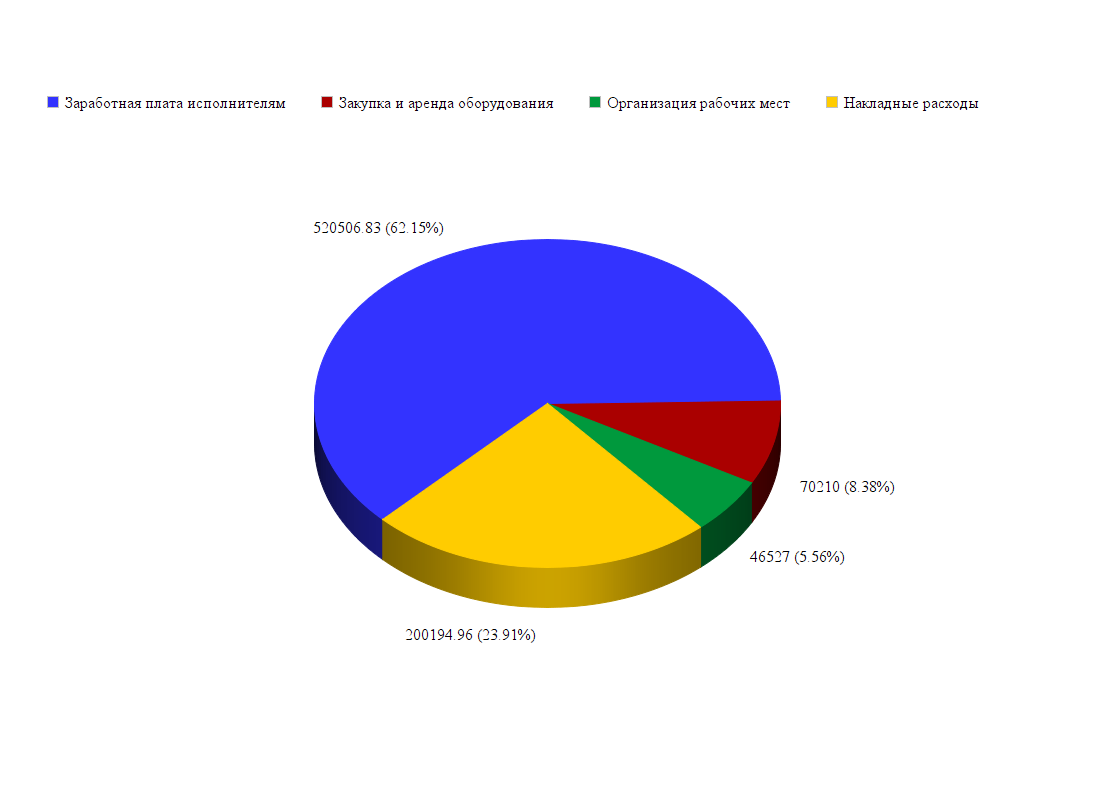
\includegraphics[scale=0.4]{pictures/circle_diagram}
\caption{Диаграмма затрат}
\label{fig:circle_diagram}
\end{figure}

\begin{table}
\caption{Суммарные затраты}
\label{table:all_expenses}
\begin{tabular} {| l | l | l | l |} 
\hline
№ & Статья расходов & Затраты, руб. & Доля, \%\\
\hline
1 &  Заработная плата исполнителям & 520506.83 & 62.15\\
\hline
2 & Закупка и аренда оборудования & 70210 & 8.38\\
\hline
3 & Организация рабочих мест & 46527 & 5.56\\
\hline
4 & Накладные расходы & 200194.96 & 23.91\\
\hline
5 & Итого & 837438.79 & 100\\
\hline
\end{tabular}
\end{table}


\section{Исследование рынка}
В разрабатываемом ПО в первую очередь заинтересованы операторы сотовых сетей и интернет-провайдеры, причем последние различных уровней, начиная от таких гигантов, как Ростелеком, оканчивая региональными филиалами.

Разрабатываемый продукт представляет собой сетевой сервис, позволяющий классифицировать трафик от L5 уровня сетевой модели и выше. Это, в свою очередь, позволяет эффективно управлять трафиком, блокировать его, настраивать сетевые экраны и т.д.

Предварительная оценка стоимости разрабатываемого ПО показала, что цена одного комплекта не будет превышать 30000 рублей.

Учитывая количество заинтересованных организаций только на территории Российской Федерации, оценим число потенциальных покупателей на годовом интервале времени $N_{P}^O$=100.


\section{Планирование цены и прогнозирование прибыли}
Частичная стоимость разработки, приходящаяся на каждый комплект ПО, определяется исходя из данных о планируемом объеме установок:
\begin{equation}
\Delta K = \frac{K} {N_{P}^O} \cdot (1+H_{\textup{СТ}}),
\end{equation}
где K - стоимость проекта, $N_{P}^O$ - планируемое число копий ПО, $H_{\textup{СТ}}$ - ставка банковского процента по долгосрочным кредитам (> 1 года).

Приняв ставку процента по долгосрочным кредитам за 24.9\% (ЗАО "Райфайзенбанк") и используя полученные ранее значения, вычислим:

$\Delta K = \frac{837438.79} {100} \cdot (1+0.249)$ = 10459.61 руб.

По результатам мониторинга рынка установим $K_{\textup{ПР}}$ = 30000 рублей. Тем самым, сумма от продаж за год составит 3000000 рублей, что обеспечит окупаемость проекта менее чем за 1 год. Определим процент прибыли от одной реализации ПО по формуле:
\begin{equation}
D_{\textup{ПРИБ}} = (\frac{K_{\textup{ПР}}} {\Delta K + K_{\textup{ВН} - 1}}) \cdot 100\%,
\end{equation}
где $K_{\textup{ВН}} = 0$ - затраты не внедрение.

Итого $D_{\textup{ПРИБ}} = 186.82\%$.

Сумма расчетной прибыли от продажи каждой установки ПО с учетом налога на добавочную стоимость $H_{\textup{НДС}} = 18\%$:
\begin{equation}
C_{\textup{ПРИБ}} = (\Delta K + K_{\textup{ВН}}) \cdot D_{\textup{ПРИБ}} \cdot (1 - H_{\textup{НДС}}) = 16023.33 руб.
\end{equation}

Для оплаты расходов на разработку ПО возьмем кредит в банке ЗАО "Райфайзенбанк" в размере 840000 рублей на срок 12 месяцев. Сумма погашения составляет 1049160 рублей. За первые 3 месяца разработки продажи равны нулю, т.к. продукт еще не разработан, при этом осуществляются выплаты заработной платы и производятся другие раннее рассчитанные расходы на разработку. В таблице~\ref{table:money_balance} приведен фрагмент общего баланса, из которого видно, что в сентябре 2016 года возможно досрочное погашение кредита.
\begin{table}
\caption{Фрагмент таблицы общего баланса}
\label{table:money_balance}
\begin{tabular} {| c | c | c | c | c | c | c |} 
\hline
Период & Баланс & Сумма & Сумма & Чистая & Баланс & Остаток\\
расчета & начальный, & продаж, & погашения & прибыль, & конечный, & по кредиту,\\
& руб & руб & кредита, руб & руб & руб & руб\\
\hline
02-04.2016 & 840000 & 0 & 262290 & -837438.79 & 2561.21 & 1049160.0\\
\hline
05.2016 & 2561.21 & 250000.0 & 87430.0 & 162570.0 & 165131.21 & 961730.0\\
\hline
06.2016 & 165131.21 & 250000.0 & 87430.0 & 162570.0 & 327701.21 & 874300.0\\
\hline
07.2016 & 327701.21 & 250000.0 & 87430.0 & 162570.0 & 490271.21 & 786870.0\\
\hline
08.2016 & 490271.21 & 250000.0 & 87430.0 & 162570.0 & 652841.21 & 699440.0\\
\hline
09.2016 & 652841.21 & 250000.0 & 87430.0 & 162570.0 & 815411.21 & 612010.0\\
\hline
\end{tabular}
\end{table}


\paragraph{Выводы}

Результаты проведенных организационно-экономических расчетов позволили оценить структуру работ и необходимое количество исполнителей. Общие затраты труда для выполнения проекта составили 65 чел/дней или 520 чел/часов. Затраты на разработку ПО составляют 837438.79 рублей.

Исходя из временных требований к реализации проекта, а также требований к квалификации персонала, была определена численность исполнителей: 2 человека - инженер и программист. По результатам построения сетевого графика и диаграммы Гантта можно сделать вывод о том, что введение дополнительных разработчиков не принесет положительного эффекта, а только увеличит затраты.

Из структуры затрат проекта видно, что основной статьей расходов является заработная плата исполнителей (62.15\%).

Для осуществления процесса разработки предполагается взять кредит в ЗАО "Райфайзенбанк" на срок 12 месяцев под 24.9\% годовых. Размер ежемесячного платежа по кредиту  составит 87430 рублей.

Стоимость 1 копии продукта составила 30000 рублей, при условии продажи 100 экземпляров в год. Планирование цены позволило спрогнозировать срок окупаемости проекта в пределах 1 года.

На основании вышеизложенного можно сделать вывод о том, что проект является экономически целесообразным.
